\documentclass[a4paper,
fontsize=11pt,
%headings=small,
oneside,
numbers=noperiodatend,
parskip=half-,
bibliography=totoc,
final
]{scrartcl}

\usepackage[babel]{csquotes}
\usepackage{synttree}
\usepackage{graphicx}
\setkeys{Gin}{width=.4\textwidth} %default pics size

\graphicspath{{./plots/}}
\usepackage[ngerman]{babel}
\usepackage[T1]{fontenc}
%\usepackage{amsmath}
\usepackage[utf8x]{inputenc}
\usepackage [hyphens]{url}
\usepackage{booktabs} 
\usepackage[left=2.4cm,right=2.4cm,top=2.3cm,bottom=2cm,includeheadfoot]{geometry}
\usepackage{eurosym}
\usepackage{multirow}
\usepackage[ngerman]{varioref}
\setcapindent{1em}
\renewcommand{\labelitemi}{--}
\usepackage{paralist}
\usepackage{pdfpages}
\usepackage{lscape}
\usepackage{float}
\usepackage{acronym}
\usepackage{eurosym}
\usepackage{longtable,lscape}
\usepackage{mathpazo}
\usepackage[normalem]{ulem} %emphasize weiterhin kursiv
\usepackage[flushmargin,ragged]{footmisc} % left align footnote
\usepackage{ccicons} 
\setcapindent{0pt} % no indentation in captions

\addto\captionsgerman{\renewcommand{\figurename}{Fig.}}

%%%% fancy LIBREAS URL color 
\usepackage{xcolor}
\definecolor{libreas}{RGB}{112,0,0}

\usepackage{listings}

\urlstyle{same}  % don't use monospace font for urls

\usepackage[fleqn]{amsmath}

%adjust fontsize for part

\usepackage{sectsty}
\partfont{\large}

%Das BibTeX-Zeichen mit \BibTeX setzen:
\def\symbol#1{\char #1\relax}
\def\bsl{{\tt\symbol{'134}}}
\def\BibTeX{{\rm B\kern-.05em{\sc i\kern-.025em b}\kern-.08em
    T\kern-.1667em\lower.7ex\hbox{E}\kern-.125emX}}

\usepackage{fancyhdr}
\fancyhf{}
\pagestyle{fancyplain}
\fancyhead[R]{\thepage}

% make sure bookmarks are created eventough sections are not numbered!
% uncommend if sections are numbered (bookmarks created by default)
\makeatletter
\renewcommand\@seccntformat[1]{}
\makeatother

% typo setup
\clubpenalty = 10000
\widowpenalty = 10000
\displaywidowpenalty = 10000

\usepackage{hyperxmp}
\usepackage[colorlinks, linkcolor=black,citecolor=black, urlcolor=libreas,
breaklinks= true,bookmarks=true,bookmarksopen=true]{hyperref}
\usepackage{breakurl}

%meta
%meta

\fancyhead[L]{K. Gietkowski\\ %author
LIBREAS. Library Ideas, 38 (2020). % journal, issue, volume.
\href{https://doi.org/10.18452/23466}{\color{black}https://doi.org/10.18452/23466}
{}} % doi 
\fancyhead[R]{\thepage} %page number
\fancyfoot[L] {\ccLogo \ccAttribution\ \href{https://creativecommons.org/licenses/by/4.0/}{\color{black}Creative Commons BY 4.0}}  %licence
\fancyfoot[R] {ISSN: 1860-7950}

\title{\LARGE{Was lebt denn da? Mikroben in mittelalterlichen Handschriften}}% title
\author{Katharina Therese Gietkowski} % author

\setcounter{page}{1}

\hypersetup{%
      pdftitle={Was lebt denn da? Mikroben in mittelalterlichen Handschriften},
      pdfauthor={Katharina Therese Gietkowski},
      pdfcopyright={CC BY 4.0 International},
      pdfsubject={LIBREAS. Library Ideas, 38 (2020).},
      pdfkeywords={Bibliothek, Handschrift, Mikroben, Analyse, Buchgeschichte},
      pdflicenseurl={https://creativecommons.org/licenses/by/4.0/},
      pdfcontacturl={http://libreas.eu},
      baseurl={http://libreas.eu},
      pdflang={de},
      pdfmetalang={de}
     }



\date{}
\begin{document}

\maketitle
\thispagestyle{fancyplain} 

%abstracts

%body
Tiere oder Lebewesen anderer Arten sind für die meisten Bibliotheken
Feinde. Nicht nur Mäuse, Ratten oder Vögel nutzen Bücher als
Nahrungsmittel oder Nistplätze und gelten somit als Schädlinge, auch
Insekten und allen voran der als Bücherwurm bekannte Holzwurm gilt als
Schrecken in Büchersammlungen. Denn die Larve des Nagekäfers frisst sich
durch hölzerne Bucheinbände und verschmäht auch die Seiten aus Papier
oder Pergament nicht. Lässt man sie lang genug gewähren, droht nicht nur
der Text durch zahlreiche Lücken unlesbar zu werden, das gesamte Buch
fällt ihm zum Opfer. Bibliothekarinnen und Restauratorinnen weltweit
sind damit beschäftigt, Lebewesen von Sammlungen fernzuhalten, um die
Kulturgüter zu bewahren.\footnote{Es wird im gesamten Artikel die
  weibliche Form verwendet, die auch die männliche miteinschließt.}

Aber keineswegs nur Tiere hinterlassen ihre Spuren, sondern natürlich
auch Menschen -- angefangen von den Herstellerinnen der verwendeten
Materialien, den Buchbinderinnen sowie den Schreiberinnen oder
Druckerinnen. Steht das Buch erst einmal in einer Bibliothek, sind es
die Leserinnen, die darin blättern und nicht selten Eselsohren oder
Notizen hinterlassen. Ob man diese Spuren als Schäden interpretiert oder
dadurch gar der Wert eines Buches steigt, wenn beispielsweise eine
berühmte Autorin ein Buch signiert, hängt jedoch vom Blickwinkel ab.

Buchwissenschaftlerinnen weltweit versuchen mit kriminalistischem
Scharfsinn Spuren dieser Art auf die Schliche zu kommen und sammeln
Indizien um herauszufinden, wer die Bücher gelesen hat
(Rezeptionsforschung), wie Bücher gelesen wurden (Leseforschung) oder
woher Bücher kommen und auf welchen Wegen sie an ihren derzeitigen
Standort gekommen sind (Provenienzforschung). Wenn Forscherinnen anhand
verschiedener Spuren die Biographien von Büchern erforschen, machen sie
auch die Bücher -- zumindest metaphorisch -- zu Lebewesen. Wie Spuren
von tierischen Buchbewohnern für die Buchwissenschaft durchaus nützlich
sein können, zeigt Ulrich Johannes Schneider anhand des Bücherwurms. Die
Larve frisst sich von den Buchdeckeln durch die Seiten und hinterlässt
Wurmlöcher und ganze Wurmgänge (Abbildunge 1). Solche Löcher
finden sich auch auf Texten oder Einzelblättern, die einst
zusammengebunden waren, jedoch im 18. und noch im 19. Jahrhundert in
zahlreichen Bibliotheken auseinandergenommen wurden. Um solche
Sammelbände, die einst Texte teils verschiedener Autorinnen und Themen
enthielten, zu rekonstruieren, könne die Buchwurmforschung als
Hilfsmittel für die Provenienzforschung dienen.\footnote{Schneider,
  Ulrich Johannes: Das Buch und sein Wurm. In: Constanze Baum, Ulrike
  Gleixner, Jörn Münkner und Hole Rößler (Hg.): Biographien des Buches.
  1. Aufl. Göttingen 2017, S. 277--290.}

Die Mikrobe gilt vor allem als Gefahr -- und das nicht nur für Bücher.
Mikroben sind Kleinstlebewesen, wie Viren, Bakterien und Pilze. Sie
verursachen besonders aufgrund der von ihnen beförderten Verbreitung von
Krankheiten Ekel und Angst -- wie wir es derzeit ganz aktuell anhand der
Pandemie erleben, die das Coronavirus auslöst. Dabei sind Mikroben ein
natürlicher Teil unserer Welt und haben nicht selten lebenswichtige
Funktionen. Ohne Mikroben könnten wir zwar problemlos den letzten
Thriller von Stephen King verdauen, nicht aber den Wein, den wir dazu
trinken.

\begin{figure}
\centering
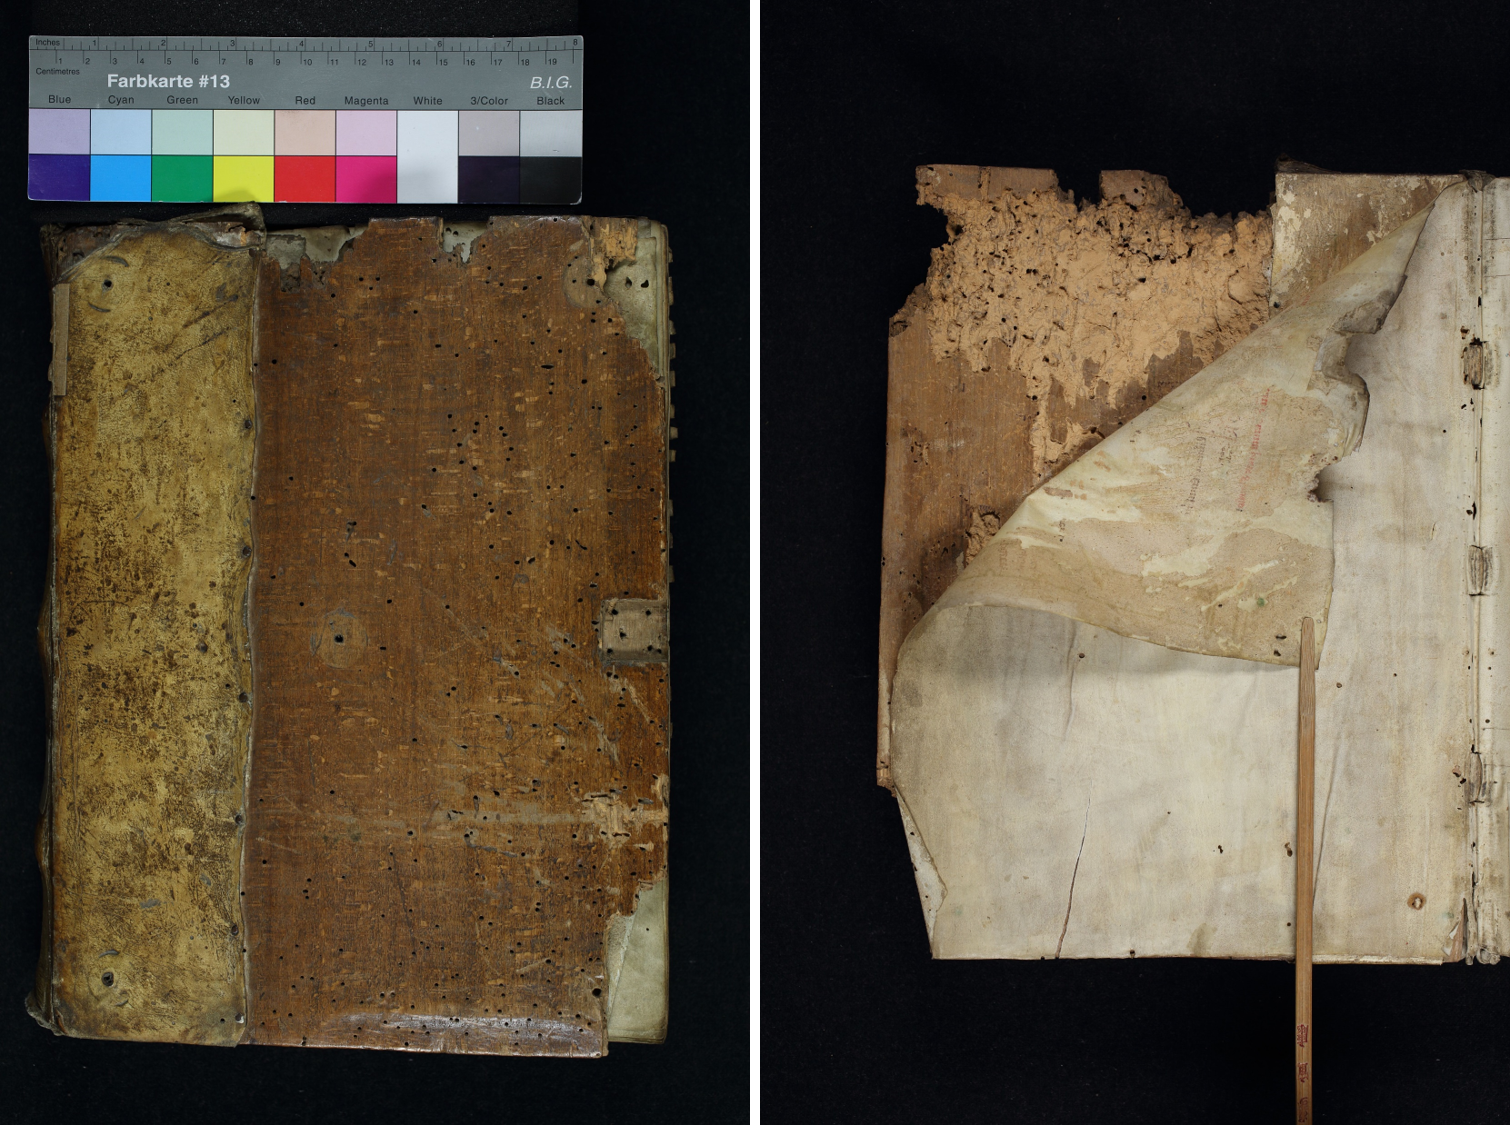
\includegraphics[width=0.9\textwidth]{img/image12.png} 
\caption{ Leipzig,
Universitätsbibliothek, MS 66: Vorder- und Rückseite des
Halbledereinbandes mit zahlreichen Fraßlöchern des Holzbocks. Weitere
Löcher, Verfärbungen und Schäden des Einbandes zeugen davon, dass der
Einband einst mit Beschlägen verziert war und eine Kette zum Schutz vor
Diebstahl angebracht war.}
\end{figure}

\hypertarget{mikroben-auf-der-spur}{%
\section{Mikroben auf der Spur}\label{mikroben-auf-der-spur}}

Mikroben sind Kosmopoliten, sie können fast alles und jeden besiedeln.
Sichtbar werden sie erst in hoher Konzentration unter dem Mikroskop. Für
das bloße Auge erkennbar ist allerdings der Schimmel, der auch das Buch
bewohnen kann. Doch auch Schimmel ist mehr als eine drohende Gefahr, die
abgewehrt werden muss. Er ist zugleich beredtes Zeugnis für die
Schicksale von Büchern. Schimmelspuren weisen darauf hin, dass ein Buch
für eine gewisse Zeit einer hohen Konzentration von Feuchtigkeit und
einer für darauf eingerichtete Mikroben angenehmen Temperatur ausgesetzt
war. Häufig sind unangemessene Lagerbedingungen dafür verantwortlich.
Schimmel kann folglich als ein Indiz angesehen werden und auf ganz
bestimmte Ereignisse im Leben eines Buches hinweisen.

Aus den Schimmelspuren der mittelalterlichen Handschrift MS 1206 in der
Universitätsbibliothek Leipzig (UBL) lässt sich noch mehr herauslesen.
Hierbei handelt es sich um eine italienische Papierhandschrift des 15.
Jahrhunderts. Zahlreiche Blätter zeugen von Wasser- und Fäulnisschäden
(Abbildung 2). Die weggefaulten Teile wurden umfangreich mit nordalpinen
Papier ausgebessert und fehlende Textstellen ergänzt. Die Fäulnisschäden
sind wahrscheinlich während des Transportes des Buches von Italien über
die Alpen nach Deutschland verursacht worden.\footnote{Mackert,
  Christoph: Leipzig, Universitätsbibliothek MS 1206. Siehe:
  \url{http://www.manuscripta-mediaevalia.de/dokumente/html/obj31569704}}
In der Frühen Neuzeit wurden Bücher in Fässern transportiert und nicht
selten sehr eng gepackt, da die Transportpreise je Fass berechnet
wurden. War das Fass undicht und ist dort einmal Wasser eingedrungen,
hatte der Schimmel ideale Bedingungen, sich über die Fracht
auszubreiten. Die medizinische Handschrift wurde dem Kloster Altzelle
von dem Freiberger Arzt Nikolaus Münzmeister vermacht, wie ein
Schenkungsvermerk ausweist. Im Zuge der Säkularisierung gelangte sie in
die Leipziger \emph{Bibliotheca Paulina} und gehört seit 1543 zum
Gründungsbestand der Universitätsbibliothek Leipzig.

\begin{figure}
\centering
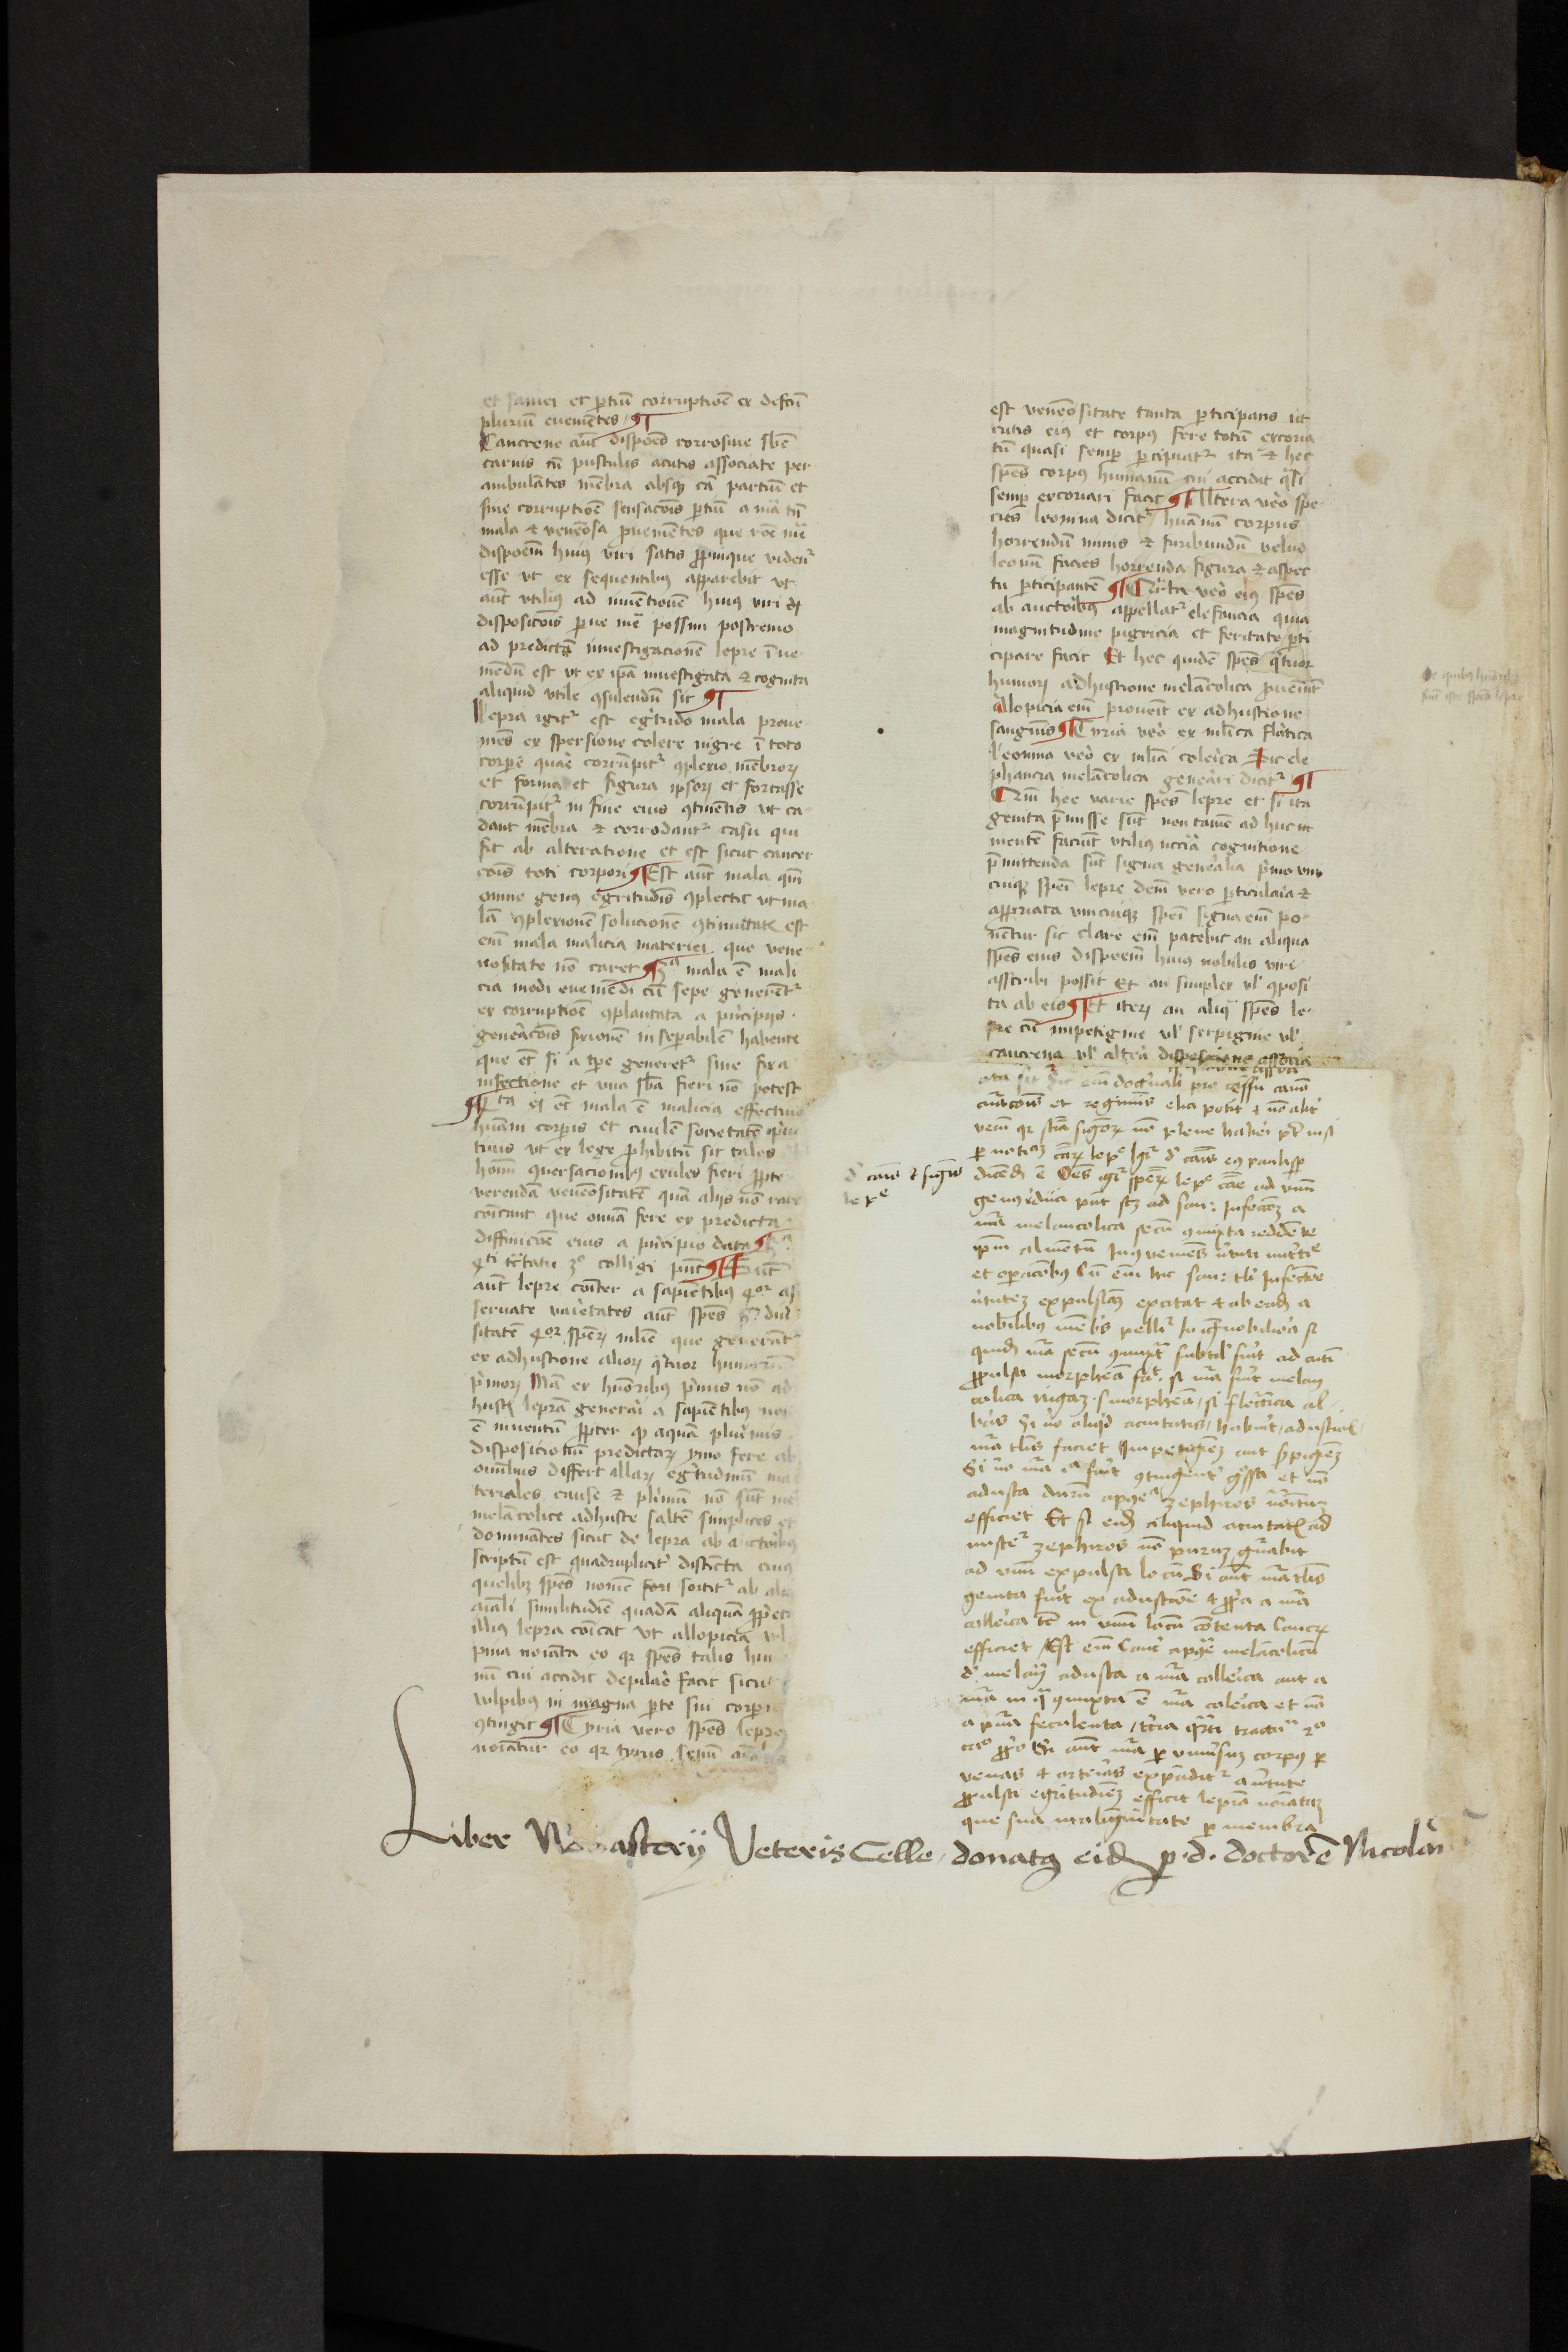
\includegraphics[width=0.85\textwidth]{img/image3.jpg}
\caption{Leipzig,
Universitätsbibliothek, Ms 1206, fol.~1v: Ausschnitt eines
ausgebesserten Blattes mit ergänztem Text sowie Beginn des
Schenkungsvermerks des Arztes Nikolaus Münzmeister.}
\end{figure}

\hypertarget{mikroben-als-sonden-der-buchbiographie}{%
\section{Mikroben als Sonden der
Buchbiographie}\label{mikroben-als-sonden-der-buchbiographie}}

Ist es also möglich, das Werk von Mikroben als Spuren zu deuten und so
die Mikroben zum Sprechen zu bringen? Können Biographien des Buches mit
Hilfe von Mikroben als Sonden neu geschrieben werden? Diese Fragen
stellt sich derzeit das Forschungsprojekt "Kontamination und Lesbarkeit
der Welt: Mikroben in Sammlungen zur Sprache bringen." Gefördert vom
BMBF und in Zusammenarbeit mit dem Handschriftenzentrum der
Universitätsbibliothek Leipzig erforschen Regina Jucknies und Katharina
Therese Gietkowski im Teilprojekt B \enquote{Mikroben als Sonden der
Buchbiographie: Kulturwissenschaftliche Objektstudien zu
Spätmittelalterlichen Sammelbänden im Bestand der Universitätsbibliothek
Leipzig}, was uns Mikroben über ihren Lebensraum Buch und dessen
Biographie berichten können. Dabei arbeiten die Leipziger Forscherinnen
zusammen mit der in Braunschweig operierenden Sammlungsphilosophie
(Teilprojekt A) und der ebendort wirkenden Mikrobiologie (Teilprojekt C)
an neuen Wegen der Lesbarkeit mittelalterlicher
Sammelhandschriften.\footnote{Das interdisziplinäre Verbundprojekt
  "Kontamination und Lesbarkeit der Welt: Mikroben in Sammlungen zur
  Sprache bringen" besteht aus dem Team des Handschriftenzentrums der
  Universitätsbibliothek Leipzig unter der Leitung von Dr.~Christoph
  Mackert und arbeitet zusammen mit dem Seminar für Philosophie der TU
  Braunschweig (Prof.~Dr.~Nicole C. Karafyllis, Dr.~Alexander Waszynski,
  Dr.~Uwe Lammers) und dem Leibniz-Institut Deutsche Sammlung von
  Mikroorganismen und Zellkulturen (DSMZ), Braunschweig (Prof.~Dr.~Jörg
  Overmann, Dr.~Cecilia Flocco). Siehe Projektseite unter:
  \url{https://www.tu-braunschweig.de/philosophie/mikrobib} Nähere
  Informationen zum Teilprojekt B (LIBER) der Universitätsbibliothek
  Leipzig siehe unter:
  \url{https://www.ub.uni-leipzig.de/forschungsbibliothek/projekte/projekte-chronologisch-alle/mikroben-als-sonden-der-buchbiographie/}}

Ziel des Teilprojektes B ist es herauszufinden, ob den zahlreichen
Methoden der Buchbiographie eine neue an die Seite gestellt werden kann.
Können mikrobielle Untersuchungen für die kulturwissenschaftliche
Forschung nutzbar gemacht werden? Um die verschiedenen Spuren in den
Handschriften zu deuten, bedarf es neben der Kenntnis zahlreicher
Methoden besonderen kriminalistischen Scharfsinns: Bei Betrachtung der
Handschriften werden vor allem durch ungewollte Spuren viele Fragen
aufgeworfen und geben zugleich Hinweise auf den Buchgebrauch: Wie kommen
Schmutz, aber auch Wolle oder Stroh in die Bücher? Sind sie Überreste
von Lesezeichen oder den Benutzungsumständen? Ist ein Fettfleck
möglicherweise durch Wachs entstanden, der von der brennenden Kerze auf
die Seite tropfte, während ein Student unter schwierigen
Lichtbedingungen den Text studierte?

\hypertarget{wie-kommt-die-mikrobe-ins-buch}{%
\section{Wie kommt die Mikrobe ins
Buch?}\label{wie-kommt-die-mikrobe-ins-buch}}

Oft ist das Wissen um das Leben der Bücher nur soweit rekonstruierbar,
wie es über Provenienzmerkmale (Spuren der Herkunft) und über weitere
Quellen wie Verzeichnisse, Kataloge oder Benutzerbücher überliefert ist.
Neben sichtbaren Spuren von Lebewesen sind es die unsichtbaren Spuren
der metaphorischen Bücherwürmer, die für die Kontamination der
Handschriften durch Mikroben verantwortlich zeichnen.

Wir kennen nie die gesamte Biographie eines Buches und wissen folglich
auch nicht immer, wann und unter welchen Umständen Mikroben überhaupt in
unsere Handschriften gekommen sind. Wer hat die Bücher aufgeschlagen,
darin geblättert, gelesen, mit ihnen gearbeitet oder gar eine Fliege
erschlagen? Es ist schwierig sich vorzustellen, durch wie viele Hände
eine Handschrift seit ihrer vollständigen Zusammensetzung zu einem
gebundenen Band bis zu ihrer heutigen Aufbewahrung im Tresorraum der UBL
gegangen ist und was ihr dabei zugestoßen ist.

Um zu versuchen, das Leben mittelalterlicher Handschriften in den
letzten Jahrhunderten nachzuvollziehen, wird an der UBL ein Blick in die
Gegenwart geworfen und das heutige Leben der Handschriften dokumentiert.
Dazu wird für den Zeitraum von drei Monaten ein im Projekt entwickeltes
Berührungsprotokoll geführt. Hierbei soll jeder, der eine Handschrift in
die Hand nimmt, dies auf einem laufenden Zettel dokumentieren, bis die
Handschrift wieder zurück an ihren Aufbewahrungsort gebracht wird.
Angefangen von der Person, die die Handschrift aus dem Magazin nimmt
(Ausheben) bis zur Benutzerin, seien es die studentischen Hilfskräfte,
die Metadaten erfassen, die wissenschaftlichen Mitarbeiterinnen, die
Handschriften katalogisieren und erforschen, die Restauratorinnen in der
Werkstatt, die Mitarbeiterinnen in der Digitalisierungswerkstatt, die
Forschenden im Lesesaal oder die Aufsichtsperson, die sie überreicht.
Jede hat einzutragen, wann und wie lange sie die Handschrift benutzt
beziehungsweise berührt hat, ebenso warum sie die Handschrift berührt
hat und welche Teile davon. So soll rekonstruiert werden, wie viele
Berührungen und damit Kontaminationen bei dem jeweiligen Geschäftsgang
(das heißt einem standardisierten und wiederkehrenden Ablauf) bei einer
Handschrift heute erfolgen. Einen ersten Eindruck in die vielfältige
Arbeit des Handschriftenzentrums der Universitätsbibliothek Leipzig gibt
ein Video, das die Digitalisierung mittelalterlicher Handschriften
beschreibt und das bereits die Vielzahl der Berührungen erahnen
lässt.\footnote{\enquote{Aus dem Tresor in die Welt. Wie das Digitalisat
  einer mittelalterlichen Handschrift entsteht}. 31.07.2020. Siehe:
  \url{https://youtu.be/P0l19JYNaj0}}

\hypertarget{biographien-mittelalterlicher-sammelbuxe4nde}{%
\section{Biographien mittelalterlicher
Sammelbände}\label{biographien-mittelalterlicher-sammelbuxe4nde}}

Das Leben eines Buches beginnt nicht erst mit seiner
Benutzung.\footnote{Zum Begriff Biographie und der Metapher des Lebens
  für die Objektforschung vgl. Regina Jucknies: Ältere Gelehrsamkeiten
  und neuere Gedankengüter. Objektbiographien lateinischer und deutscher
  Sammelhandschriften der UB Leipzig. In: Sabine Walther u.a. (Hgg.):
  Res, Artes et Religio. Essays in Honor of Rudolf Simek. Leeds: 2020.}
Zur Biographie gehört bereits die Herstellung der verwendeten
Materialien wie Papier, Pergament, Tinten und Farben für die
Buchmalereien, Initialen und Rubrizierungen. Häufig werden aus
Kostengründen mehrere Texte sogar verschiedener Formate zusammengebunden
(Abbildung 3). Der verwendete, einfache oder mit Leder überzogene, teils
ausgeschmückte (Holz-)Einband schützt die Materialien vor Schmutz und
Feuchtigkeit und dient als Träger von Zeichen seiner Herkunft, darunter
Namen ehemaliger Besitzerinnen oder Signaturen der besitzenden
Institutionen. Der Herstellung folgt das aktive Leben der Bücher.
Handschriften haben oft viele Reisen unternommen und lagen oder standen
auf vielen Regalen, Tischen und in Kisten, ehe sie an ihren derzeitigen
Standort gekommen sind. Sie überlebten vielleicht Katastrophen wie
Brände, Kriege und Fluten. Einige Lebensstationen sind mit dem bloßen
Auge sichtbar, einige Merkmale sprechen für sich, die meisten aber sind
Indizien, die gelesen und gedeutet werden müssen. Das erfordert neue
Ansätze, neue Sichtweisen, neue Einschätzungen. Die Spurensuche in
mittelalterlichen Handschriften im Rahmen des vom BMBF geförderten
Projektes wird ab März 2021 in einer Ausstellung an der
Universitätsbibliothek Leipzig gezeigt, zu der auch ein Katalog
erscheinen wird.

\begin{figure}
\centering
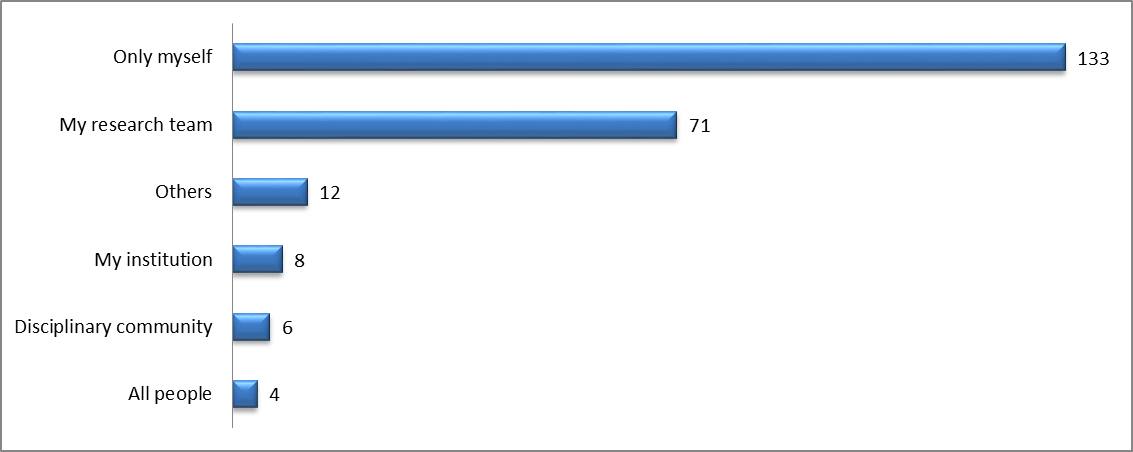
\includegraphics[width=0.9\textwidth]{img/image4.jpg}
\caption{Leipzig,
Universitätsbibliothek, Ms 768 (Foto: Olaf Mokansky): In diesem Einband
sind Texte unterschiedlicher Herkunft und Größe zusammengebunden.}
\end{figure}

\hypertarget{literatur}{%
\section{Literatur}\label{literatur}}

Jucknies, Regina: Ältere Gelehrsamkeiten und neuere Gedankengüter.
Objektbiographien lateinischer und deutscher Sammelhandschriften der UB
Leipzig. In: Sabine Walther u.a. (Hgg.): Res, Artes et Religio. Essays
in Honor of Rudolf Simek. Leeds 2020. (In Druck)

Mackert, Christoph: Bartholomaeus Montagna, Consilia medica.
Universitätsbibliothek Leipzig MS 1206. Siehe:
\url{http://www.manuscripta-mediaevalia.de/dokumente/html/obj31569704}

Schneider, Ulrich Johannes: Das Buch und sein Wurm. In: Constanze Baum,
Ulrike Gleixner, Jörn Münkner und Hole Rößler (Hgg.): Biographien des
Buches. 1. Aufl. Göttingen 2017, S. 277--290.

%autor
\begin{center}\rule{0.5\linewidth}{0.5pt}\end{center}

\textbf{Katharina Therese Gietkowski} studierte Kunstgeschichte,
Anglistik, Buchwissenschaft und Textforschung sowie Europäische
Ethnologie an der Westfälischen Wilhelms-Universität Münster und der
Università Suor Orsola Benincasa in Neapel. Es folgte ein Masterstudium
der Bibli\-otheks- und Informationswissenschaft an der Hochschule für
Technik, Wirtschaft und Kultur (HTWK) in Leipzig. Von 2014 bis 2015 war
sie an der Herzog August Bibliothek Wolfenbüttel als wissenschaftliche
Bibliothekarin in der Abteilung Alte Drucke tätig. Seit 2015 promoviert
Katharina Gietkowski im Graduiertenkolleg "Wissensspeicher und
Argumentationsarsenal. Funktionen der Bibliothek in den kulturellen
Zentren im Europa der Frühen Neuzeit" am IKFN der Universität
Osnabrück. Als wissenschaftliche Mitarbeiterin arbeitet sie seit 2019 im
Handschriftenzentrum der Universitätsbibliothek Leipzig im
BMBF-Teilprojekt "Mikroben als Sonden der
Buchbiographie. Kulturwissenschaftliche Objektstudien zu
Spätmittelalterlichen Sammelbänden im Bestand der Universitätsbibliothek
Leipzig."

\end{document}
